\documentclass[tikz,border=15pt]{standalone}
\usepackage[T1]{fontenc}
\usepackage{tgheros}
\usepackage{sfmath}
\usepackage{amsmath}
\usepackage{tikz}
\usetikzlibrary{arrows.meta,positioning,shapes.geometric,fit,backgrounds,calc}
\usepackage{xcolor}

\renewcommand{\familydefault}{\sfdefault}

% Harvard Crimson & ETH Zurich Academic Semantic Palette
\definecolor{harvardcrimson}{HTML}{A51C30}
\definecolor{ethdarkblue}{HTML}{1F407A}
\definecolor{ethblue}{HTML}{215CAF}
\definecolor{ethpetrol}{HTML}{007A87}
\definecolor{ethbronze}{HTML}{B87333}
\definecolor{ethpurple}{HTML}{5B4B8A}
\definecolor{ethslate}{HTML}{475569}
\definecolor{cardbg}{HTML}{F8FAFC}
\definecolor{cardborder}{HTML}{CBD5E1}
\definecolor{safeTeal}{HTML}{10B981}

\begin{document}
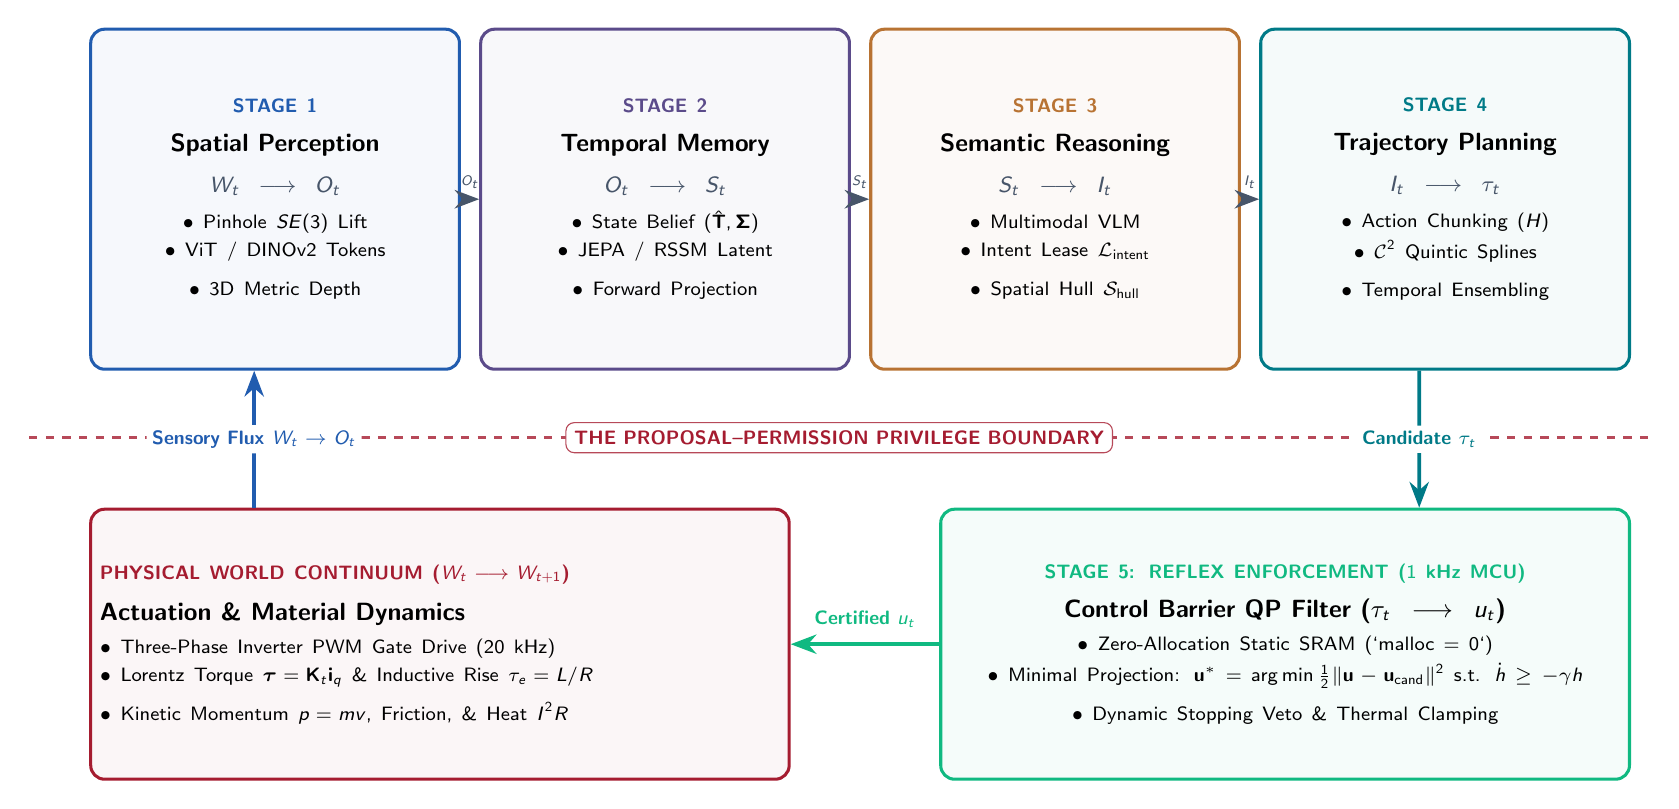
\begin{tikzpicture}[
  font=\sffamily,
  >=Stealth,
  stagecard/.style={
    draw=cardborder,
    fill=white,
    rounded corners=5pt,
    line width=1.1pt,
    text width=1.65in,
    minimum height=1.70in,
    inner sep=7pt,
    align=center,
    anchor=north west
  },
  dataarrow/.style={
    ->,
    line width=1.3pt,
    draw=ethslate
  },
  boundaryline/.style={
    draw=harvardcrimson!80,
    dashed,
    line width=1.1pt
  }
]

  % -------------------------------------------------------------
  % TOP ROW: STAGES 1, 2, 3, 4 (PROPOSAL REALM)
  % -------------------------------------------------------------

  % Stage 1: Spatial Perception
  \node[stagecard, draw=ethblue, fill=ethblue!4] (s1) at (0.0in, 0.0in) {
    {\scriptsize\bfseries\color{ethblue} STAGE 1}\\[2pt]
    {\small\bfseries Spatial Perception}\\[3pt]
    {\footnotesize\color{ethslate}$W_t \longrightarrow O_t$}\\[5pt]
    {\scriptsize $\bullet$ Pinhole $SE(3)$ Lift\\[2pt]
    $\bullet$ ViT / DINOv2 Tokens\\[2pt]
    $\bullet$ 3D Metric Depth}
  };

  % Stage 2: Temporal Memory
  \node[stagecard, draw=ethpurple, fill=ethpurple!4] (s2) at (1.95in, 0.0in) {
    {\scriptsize\bfseries\color{ethpurple} STAGE 2}\\[2pt]
    {\small\bfseries Temporal Memory}\\[3pt]
    {\footnotesize\color{ethslate}$O_t \longrightarrow S_t$}\\[5pt]
    {\scriptsize $\bullet$ State Belief $(\hat{\mathbf{T}}, \mathbf{\Sigma})$\\[2pt]
    $\bullet$ JEPA / RSSM Latent\\[2pt]
    $\bullet$ Forward Projection}
  };

  % Stage 3: Semantic Reasoning
  \node[stagecard, draw=ethbronze, fill=ethbronze!4] (s3) at (3.90in, 0.0in) {
    {\scriptsize\bfseries\color{ethbronze} STAGE 3}\\[2pt]
    {\small\bfseries Semantic Reasoning}\\[3pt]
    {\footnotesize\color{ethslate}$S_t \longrightarrow I_t$}\\[5pt]
    {\scriptsize $\bullet$ Multimodal VLM\\[2pt]
    $\bullet$ Intent Lease $\mathcal{L}_{\text{intent}}$\\[2pt]
    $\bullet$ Spatial Hull $\mathcal{S}_{\text{hull}}$}
  };

  % Stage 4: Trajectory Planning
  \node[stagecard, draw=ethpetrol, fill=ethpetrol!4] (s4) at (5.85in, 0.0in) {
    {\scriptsize\bfseries\color{ethpetrol} STAGE 4}\\[2pt]
    {\small\bfseries Trajectory Planning}\\[3pt]
    {\footnotesize\color{ethslate}$I_t \longrightarrow \tau_t$}\\[5pt]
    {\scriptsize $\bullet$ Action Chunking ($H$)\\[2pt]
    $\bullet$ $\mathcal{C}^2$ Quintic Splines\\[2pt]
    $\bullet$ Temporal Ensembling}
  };

  % Connecting Arrows across Top Row
  \draw[dataarrow] (s1.east) -- (s2.west)
    node[midway, above, font=\tiny\bfseries\color{ethslate}] {$O_t$};
  \draw[dataarrow] (s2.east) -- (s3.west)
    node[midway, above, font=\tiny\bfseries\color{ethslate}] {$S_t$};
  \draw[dataarrow] (s3.east) -- (s4.west)
    node[midway, above, font=\tiny\bfseries\color{ethslate}] {$I_t$};

  % -------------------------------------------------------------
  % PROPOSAL-PERMISSION BOUNDARY
  % -------------------------------------------------------------
  \draw[boundaryline] (-0.30in, -2.05in) -- (7.80in, -2.05in);
  \node[font=\sffamily\bfseries\scriptsize, fill=white, draw=harvardcrimson!80, rounded corners=3pt, inner sep=3pt, text=harvardcrimson] at (3.75in, -2.05in) {
    THE PROPOSAL--PERMISSION PRIVILEGE BOUNDARY
  };

  % -------------------------------------------------------------
  % BOTTOM ROW: STAGE 5 (PERMISSION & REFLEX) & PHYSICAL WORLD
  % -------------------------------------------------------------

  % Physical World Block (Left)
  \node[draw=harvardcrimson, fill=harvardcrimson!4, rounded corners=5pt, line width=1.1pt, text width=3.40in, minimum height=1.35in, anchor=north west] (pworld) at (0.0in, -2.40in) {
    {\scriptsize\bfseries\color{harvardcrimson} PHYSICAL WORLD CONTINUUM ($W_t \longrightarrow W_{t+1}$)}\\[3pt]
    {\small\bfseries Actuation \& Material Dynamics}\\[4pt]
    {\scriptsize $\bullet$ Three-Phase Inverter PWM Gate Drive ($20\text{ kHz}$)\\[2pt]
    $\bullet$ Lorentz Torque $\boldsymbol{\tau} = \mathbf{K}_t \mathbf{i}_q$ \& Inductive Rise $\tau_e = L/R$\\[2pt]
    $\bullet$ Kinetic Momentum $p=mv$, Friction, \& Heat $I^2 R$}
  };

  % Stage 5: Reflex Enforcement (Right)
  \node[stagecard, draw=safeTeal, fill=safeTeal!4, text width=3.25in, minimum height=1.35in, anchor=north west] (s5) at (4.25in, -2.40in) {
    {\scriptsize\bfseries\color{safeTeal} STAGE 5: REFLEX ENFORCEMENT ($1\text{ kHz}$ MCU)}\\[2pt]
    {\small\bfseries Control Barrier QP Filter ($\tau_t \longrightarrow u_t$)}\\[4pt]
    {\scriptsize $\bullet$ Zero-Allocation Static SRAM (`malloc = 0`)\\[2pt]
    $\bullet$ Minimal Projection: $\mathbf{u}^* = \arg\min \frac{1}{2}\|\mathbf{u} - \mathbf{u}_{\text{cand}}\|^2 \text{ s.t. } \dot{h} \ge -\gamma h$\\[2pt]
    $\bullet$ Dynamic Stopping Veto \& Thermal Clamping}
  };

  % Downward Proposal Arrow from Stage 4 to Stage 5
  \draw[dataarrow, draw=ethpetrol, line width=1.4pt] ($(s4.south west) + (0.80in, 0)$) -- ($(s5.north west) + (2.40in, 0)$)
    node[midway, fill=white, inner sep=2pt, rounded corners=2pt, font=\scriptsize\bfseries\color{ethpetrol}] {Candidate $\tau_t$};

  % Arrow from Stage 5 to Physical World
  \draw[dataarrow, draw=safeTeal, line width=1.4pt] (s5.west) -- (pworld.east)
    node[midway, above=2pt, font=\scriptsize\bfseries\color{safeTeal}] {Certified $u_t$};

  % Endogenous Feedback Arrow from Physical World up to Stage 1
  \draw[dataarrow, draw=ethblue, line width=1.4pt] ($(pworld.north west) + (0.825in, 0)$) -- ($(s1.south west) + (0.825in, 0)$)
    node[midway, fill=white, inner sep=2pt, rounded corners=2pt, font=\scriptsize\bfseries\color{ethblue}] {Sensory Flux $W_t \to O_t$};

\end{tikzpicture}
\end{document}
